\section{noethersche Ringe}

Sei $R$ ein Ring.

\begin{definition}[endlich erzeugt, noethersch]
	\begin{enumerate}[label=(\alph*)]
		\item Ein Ideal $I\unlhd R$ ist \begriff[Ideal!]{endlich erzeugt}, wenn $I=\langle A\rangle$ mit $A\subseteq R$ endlich.
		\item Der Ring $R$ ist \begriff{noethersch}, wenn jedes Ideal $I\unlhd R$ endlich erzeugt ist.
	\end{enumerate}
\end{definition}

\begin{example}
	$R$ Hauptidealring $\Rightarrow R$ noethersch
\end{example}

\begin{example}
	$\ratio[x_1,x_2,...] = \ratio[x_i\mid i\in\natur]$ ist nicht noethersch.
	\begin{align}
		I = (x_1,x_2,...) = \langle\{x_i\mid i\in\natur \}\rangle\notag
	\end{align}
\end{example}
\begin{proof}
	Wäre $I=(f_1,...,f_r)$ so existiert ein $n\in\natur$ mit $f_1,...,f_r\in\ratio[x_1,...,x_n]$. Dann ist $x_{n+1}\notin (f_1,...,f_r)=I$. Angenommen $x_{n+1}\in (f_1,...,f_r)\Rightarrow x_{n+1}=\sum_{i=1}^{r} g_if_i$ mit $g_i\in\ratio[x_1,x_2,...]$. Nach  der universellen Eigenschaft existiert ein Homomorphismus $\phi:\ratio[x_1,x_2,...]\to\ratio[x_1,x_2,...]$ mit $\phi\vert_\ratio = \id_\ratio$, $\phi(x_i)=x_i$ für $i\neq n+1$ und $\phi(x_{n+1})=1$. \\
	$\Rightarrow 1 = \phi(x_{n+1}) = \phi(\sum g_if_i) = \sum\phi(g_i)f_i\in I$ \\
	$\Rightarrow 1 = \sum_{i=1}^m h_ix_i$ mit $h_i\in\ratio[x_1,x_2,...]$ \\
	Nach der universellen Eigenschaft existiert ein Homomorphismus $\psi$ mit $\psi\vert_\ratio = \id_\ratio$ und $\psi(x_i) = 0\quad\forall i$ \\
	$\Rightarrow 1 = \psi(1) = \psi(\sum h_ix_i) = \sum\psi(h_i)\cdot 0 = 0\Rightarrow$ Widerspruch!
\end{proof}

\begin{proposition}
	\proplbl{2_9_4}
	Es sind äquivalent:
	\begin{enumerate}[label=(\alph*)]
		\item $R$ ist noethersch
		\item Jede aufsteigende Kette von Idealen
		\begin{align}
			I_1 \subseteq I_2 \subseteq I_3 \subseteq\dots\notag
		\end{align}
		wird \begriff{stationär}, das heißt es existiert ein $n\in\natur$ mit $\forall i\ge n: I_i=I_{i+1}$. (\begriff{aufsteigende Kettenbedingung})
		\item Jede nichtleere Menge von Idealen von $R$ besitzt ein bezüglich Inklusion maximales Element.
	\end{enumerate}
\end{proposition}
\begin{proof}
	\begin{itemize}
		\item (a) $\Rightarrow$ (b): $I=\bigcup I_n$ ist ein Ideal von $R$, vgl. \propref{2_2_13} $\xRightarrow{(a)} I = (x_1,...,x_k)$ mit $x_1,...,x_k\in I$. Für jedes $i=1,...,k$ ist $x_i\in I_{n_i}$ für ein $n_i$. Mit $n=\max\{n_1,...,n_k\}$ ist dann $x_i\in I_n$ für alle $i$. \\
		$\Rightarrow I = (x_1,...,x_k) \subseteq I_n \subseteq I_{n+1}\subseteq \dots\subseteq I$ \\
		$\Rightarrow I_n = I_{n+1} = \dots$
		\item (b) $\Rightarrow$ (c): Sei $\mathcal{J}$ eine Menge von Idealen von $R$. Angenommen $\mathcal{J}$ habe kein maximales Element. Wähle $I_1\in\mathcal{J}$. Da $I_1$ nicht maximal ist, existiert $I_1\subsetneqq I_2\in\mathcal{J}$. Da $I_2$ nicht maximal ist, existiert $I_2\subsetneqq I_3\in\mathcal{J}$, etc. Wir erhalten eine aufsteigende Kette $I_1\subsetneqq I_2\subsetneqq I_3\subsetneqq\dots$ von Idealen von $R$ im Widerspruch zu (b).
		\item (c) $\Rightarrow$ (a): Sei $I\unlhd R$. Definiere $\mathcal{J} = \{J\unlhd R\mid J\subseteq I, J\text{ endlich erzeugt}\}$. Da $(0)\in\mathcal{J}$ ist $\mathcal{J}\neq \emptyset$, nach (c) existiert deshalb ein maximales Ideal $J\in\mathcal{J}$. $J\in\mathcal{J}\Rightarrow J=(x_1,...,x_k)$ mit $x_1,...,x_k\in I$. Wäre $J\subsetneqq I$, so wähle $a\in I\setminus J\Rightarrow J'=(x_1,...,x_k,a)\in\mathcal{J}$, aber $J\subsetneqq J'$, im Widerspruch zur Maximalität von $J$. Somit ist $I=J$ endlich erzeugt.
	\end{itemize}
\end{proof}

\begin{conclusion}
	\proplbl{2_9_5}
	$R$ noethersch, $I\unlhd R\Rightarrow \lnkset{R}{I}$ noethersch
\end{conclusion}
\begin{proof}[Variante 1]
	$J\unlhd R\setminus I\Rightarrow \pi_I^{-1}(J)\unlhd R\Rightarrow\pi_I^{-1}(J)=(x_1,...,x_k)$ endlich erzeugt $\Rightarrow J=\pi_I(\pi_I^{-1}(J)) = (\pi_I(x_1),...,\pi_I(x_k))$ ist endlich erzeugt.
\end{proof}
\begin{proof}[Variante 2]
	\propref{2_9_4}(b) + \propref{2_2_9}
\end{proof}

\begin{theorem}[\person{Hilbert}'scher Basissatz, 1890]
	$R$ noethersch $\Rightarrow R[x]$ noethersch
\end{theorem}
\begin{proof}
	Sei $I\unlhd R[x]$. Für $n\in\natur_0$ definiere $I_n = \{\LC(f)\mid f\in I,\deg(f)=n\}\cup \{0\}$. Dann ist $I_n\unlhd R$:
	\begin{itemize}
		\item $0\neq a_n\in I_n$, $r\in R\Rightarrow a=\LC(f)$, $f\in I$, $\deg(f)=n$ \\
		$\Rightarrow ra=0$ oder [$ra=\LC(rf)$, $rf\in I$, $\deg(rf)=n$] \\
		$\Rightarrow ra\in I_n$
		\item $a,b\in I_n\Rightarrow a=\LC(f)$, $b=\LC(g)$, $f,g\in I$, $\deg(f)=\deg(g)=n$ \\
		$\Rightarrow a+b=0$ oder  [$a+b=\LC(f+g)$, $f+g\in I$, $\deg(f+g)=n$] \\
		Auch dann ist $I_n\subseteq I_{n+1}\quad\forall n$, denn $a\in I_n\Rightarrow a = \LC(f)$, $f\in I$, $\deg(f)=n\Rightarrow a=\LC(x\cdot f)$, $x\cdot f\in I$, $\deg(x\cdot f)=n+1\Rightarrow a\in I_n$ 
	\end{itemize}
	Da $R$ noethersch ist, wird die Kette
	\begin{align}
		I_0 \subseteq I_1\subseteq \dots \notag
	\end{align}
	stationär, es existiert also ein $n_0$ mit
	\begin{align}
		I_{n_0} = I_{n_0+1} = \dots\notag
	\end{align}
	Da $R$ noethersch ist und $I_0,...,I_{n_0}$ endlich erzeugt. Für $n=0,...,n_0$ wähle $f_{n,1},...,f_{n,k_n}\in I$ mit $\deg(f_{n,i})=n$ und 
	\begin{align}
		I_n = (\LC(f_{n,1}),...,\LC(f_{n,k_n})) \notag
	\end{align}
	Definiere $J=\langle \{f_{n,i}\mid  n=0,...,n_0,i=1,...,k_n\}\rangle\unlhd R[x]\Rightarrow J\subseteq I$. Wir wollen nun zeigen, dass $J=I$. Sei dazu $g\in I$. Induktion nach $d=\deg(g)$. \\
	\emph{$d=-\infty$:} klar \\
	\emph{$d\ge 0$:} Setze $a=\LC(g)$, $n=\min\{g,n_0\}$. $a\in I_d=I_n$ \\
	$\Rightarrow a = \sum_{i=1}^{k_n} r_i\LC(f_{n,i})$, $r_1,...,r_{k_n}\in R$\\
	$\Rightarrow f = \sum_{i=1}^{k_n} r_i f_{n,i}\in J$, $\LC(f) = \sum_{i=1}^{k_n} r_i\LC(f_i)=a\neq 0$ \\
	$\Rightarrow g_1 = g - x^{d-n}f\in I$, $\deg(g_1)<d$ \\
	$\xRightarrow{I.H.} g_1\in J\Rightarrow g = g_1+x^{d-n}\in J$
\end{proof}

\begin{conclusion}
	\proplbl{2_9_7}
	$R$ noethersch $\Rightarrow R[x_1,...,x_n]$ noethersch
\end{conclusion}

\begin{conclusion}
	$R$ noethersch, $R\subseteq S$ endlich erzeugte Ringerweiterung, das heißt es existieren $x_1,...,x_n\in S$ mit: Ist $R\cup \{x_1,...,x_n\}\subseteq S_0\subseteq S$ Teilring, so ist $S=S_0$. Dann ist $S$ noethersch.
\end{conclusion}
\begin{proof}
	Nach der universellen Eigenschaft existiert ein Homomorphismus $\phi:R[x_1,...,x_n]\to S$ mit $\phi\vert_R = \id_S$ und $\phi(x_i)=x_i\quad\forall i$. $\Image(\phi)\supseteq R\cup \{x_1,...,x_n\}$ ist Teilring von $S$. \\
	$\Rightarrow \phi$ ist surjektiv \\
	$\Rightarrow S\cong \lnkset{R[x_1,...,x_n]}{\Ker(\phi)}$ \\
	$R$ noethersch $\xRightarrow{\propref{2_9_7}} R[x_1,...,x_n]$ noethersch $\xRightarrow{\propref{2_9_5}} \lnkset{R[x_1,...,x_n]}{\Ker(\phi)}$ noethersch
\end{proof}

\begin{example}
	\proplbl{2_9_9}
	Ist $K$ ein Körper so ist $K[x_1,...,x_n]$ noethersch, aber für $n>1$ kein Hauptidealring.
\end{example}

\begin{example}
	Für $n\in\whole$ ist $\whole[\sqrt{n}] = \{a+b\sqrt{n}\mid a,b\in\whole\}\subseteq\comp$ ist Teilring und $\whole\subseteq\whole[\sqrt{n}]$ ist endlich erzeugt $\xRightarrow{\propref{2_9_9}}\whole[\sqrt{n}]$ ist noethersch, aber zum Beispiel für $n=-5$ nicht einmal faktoriell.
\end{example}

\begin{example}
	Ist $K$ ein Körper, so ist $K[x_1,x_2,...]$ faktoriell (Übung!) aber nicht noethersch.
\end{example}

\begin{remark}
	Es gilt:
	\begin{center}
		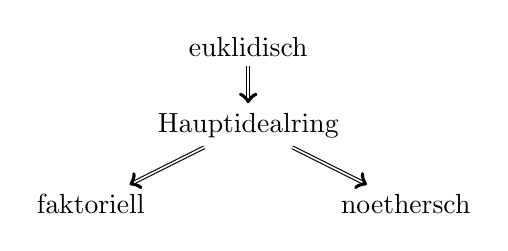
\begin{tikzpicture}
			\node at (0,0) (a) {euklidisch};
			\node at (0,-1) (b) {Hauptidealring};
			\node at (-2,-2) (c) {faktoriell};
			\node at (2,-2) (d) {noethersch};
			\draw[->,double] (a) -- (b);
			\draw[->,double] (b) -- (c);
			\draw[->,double] (b) -- (d);
		\end{tikzpicture}
	\end{center}
	und es gelten keine weiteren Implikationen.
\end{remark}

\begin{remark}
	Es gilt:
	\begin{center}
		\begin{tabular}{p{4cm}|p{4cm}|p{5cm}}
			$R$ & $\lnkset{R}{I}$ & $R[x]$ \\
			\hline
			Hauptidealring & $\checkmark$ & $\times$ \\
			faktoriell & $\times$ & $\checkmark$ (Satz von \person{Gauss}) \\
			noethersch & $\checkmark$ & $\checkmark$ (\person{Hilbert}'scher Basissatz)
		\end{tabular}
	\end{center}
\end{remark}